\newpage
\sectiontitledouble{4.) Qualitative Assessment}{by the Faculty Member}
\fakesection{Qualitative Assessment by the Faculty Member}

%Candidates for tenure and promotion should prepare a statement that reflects their own assessment of their teaching, research/creative achievement, and service. Identify any accomplishments associated with or resulting from teaching, research/creative achievement, and service. This statement is the place for the candidate to provide informative commentary on the criteria for promotion and tenure and his or her assessment on how the criteria have been achieved. The assessment should indicate the impact, significance, or value of the work. Candidates should provide clear and sufficient information about their individual roles in collaborative projects, publications, presentations, or grants. In addition, the statement should include specific plans for continuation of the candidate’s research or creative activity agenda, plans to enhance teaching effectiveness, and future participation in service to the University and/or profession. Any service directly provided to external communities must show causal relationship to the University.
%You may use the following questions as a guide.
%Teaching:
%i. How did your teaching develop over the review period?
%ii. Assess the strengths/weaknesses of your teaching and indicate what steps you have taken to improve the quality of the instruction you offer students.
%iii. How has your field changed and how do your courses reflect those changes?
%iv. Whatisespeciallyinnovativeaboutyourcourses?
%v. How do you attend to and measure student learning?
%vi. Howdoyourcoursesplayaroleinachievingdepartmentalorinstitutionalgoals?
%vii. How does your teaching connect to other forms of scholarship?
%viii.What questions do you ask of your own teaching?
%ix. What are your scholarly practices regarding teaching (inquiry, reading, collaboration, revision)?
%x. What texts or theories have influenced the ways you think about your discipline, the students you teach, and the ways you design your courses?
%xi. Howhasnewlearningofyourown(suchasscholarlyinterests,expertisewithtechnology, community engagement) affected your courses and your students’ learning?
%Research:
%i. How did your research/creative activity develop over the review period?
%ii. Assess your research contribution or creative activity with respect to the relevant community (such as scientific community) in general.
%iii. What specific contributions do your research and creative achievements make to your academic discipline?
%iv. How has your research/creative activity helped to benefit you, your department, students, and the institution?
%v. Why do you think your research/creative activity and scholarly work is at the level of your peers in your field of expertise?
%vi. HowdoyouthinkyourgrantshelptoimprovetheUniversity’scapabilities?
%vii. What professional affiliations do you actively engage in membership and how does that contribute to your field or discipline?
%viii.Describe your near future and long-term plans or directions regarding the research/creative activity.
%Service:
%i. Identify University, professional and community groups and/or organizations with which you are working. Describe the nature of the organization(s) and explain your role and/or office within the organization(s).
%ii. Identify your participation in these service organizations and indicate the scope and nature of the efforts.
%iii. What leadership role(s) have you taken in service organizations? What specific accomplishments were achieved under your leadership?
%iv. For University service, describe your responsivity to the institutional needs.
%v. For professional and community service, describe your responsivity to the group’s mission or efforts.
%vi. How have your services benefitted the community and the institution?
%vii. Provide you near future and long term plans or directions with respect to services
%The following sections generally consist of supporting documentation related to teaching, research, and service. External support letters provided as evidence should be from persons who have direct knowledge of candidate’s contribution and can offer verification of the candidate’s qualitative statement.

\newpage

\subsection{Introduction}
\blindtext

\subsection{Research}
\blindtext

\subsection{Teaching}
\blindtext


\begin{quotation}
``{\it \small Here is a sample quotation: \blindtext}''
\end{quotation}

%
\begin{figure}[H]
\caption{Here is a sample figure.}
\centering
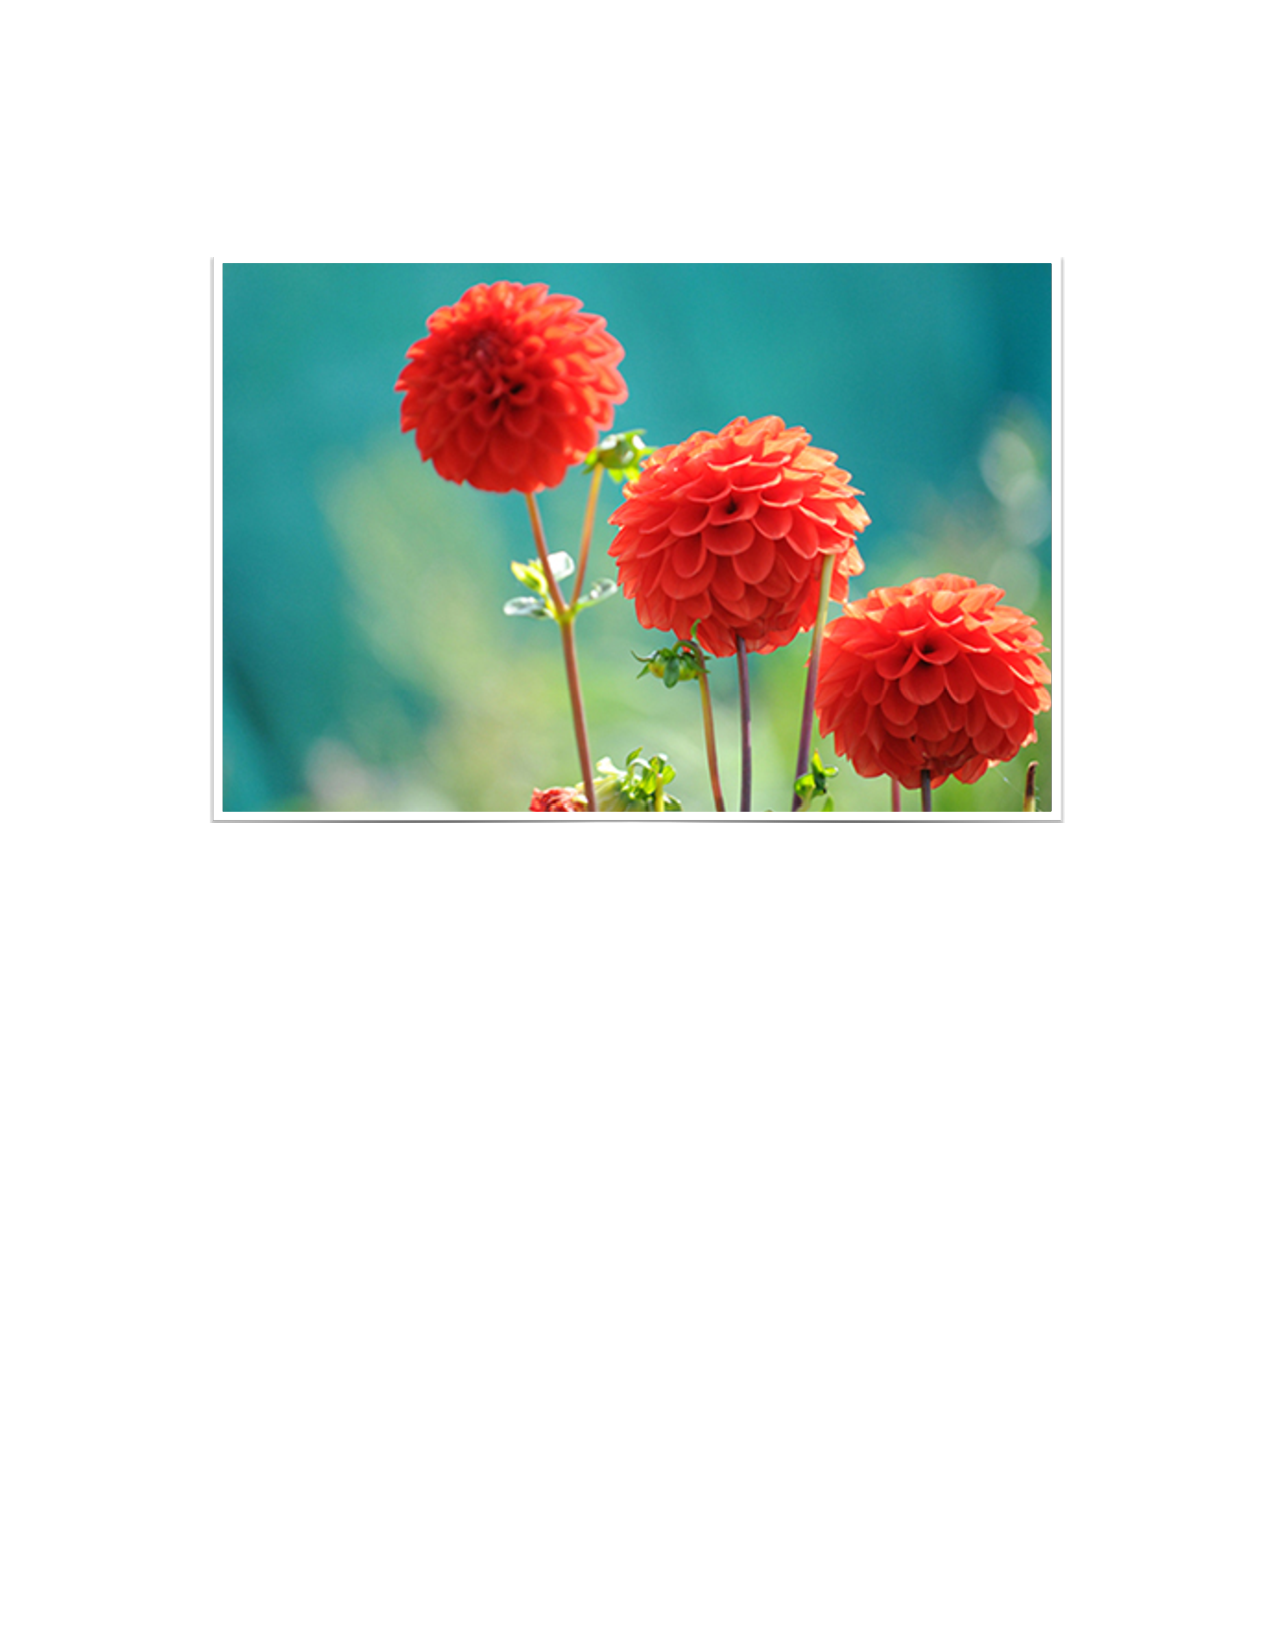
\includegraphics[width=0.5\textwidth]{Files/4_Qualitative_Assessment/Fig.pdf}
\label{fig_label}
\end{figure}




\subsection{Service}
\blindtext


\subsection{Summary}
\blindtext
